\documentclass[letterpaper,11pt]{article}
\oddsidemargin -1.0cm \textwidth 17.5cm

\usepackage[utf8]{inputenc}
\usepackage[activeacute,spanish, es-lcroman]{babel}
\decimalpoint
\usepackage{amsfonts,setspace}
\usepackage{amsmath}
\usepackage{amssymb, amsmath, amsthm}
\usepackage{comment}
\usepackage{float}
\usepackage{amssymb}
\usepackage{dsfont}
\usepackage{anysize}
\usepackage{multicol}
\usepackage{enumerate}
\usepackage{graphicx}
\usepackage[left=1.5cm,top=2cm,right=1.5cm, bottom=1.7cm]{geometry}
\setlength\headheight{1.5em} 
\usepackage{fancyhdr}
\usepackage{multicol}
\usepackage{hyperref}
\usepackage{wrapfig}
\usepackage{subcaption}
\usepackage{siunitx}
\usepackage{cancel}
\usepackage{mdwlist}
\usepackage{svg}
\pagestyle{fancy}
\fancyhf{}
\renewcommand{\labelenumi}{\normalsize\bfseries P\arabic{enumi}.}
\renewcommand{\labelenumii}{\normalsize\bfseries (\alph{enumii})}
\renewcommand{\labelenumiii}{\normalsize\bfseries \roman{enumiii})}


\begin{document}

\fancyhead[L]{\itshape{Facultad de Ciencias F\'isicas y Matem\'aticas}}
\fancyhead[R]{\itshape{Universidad de Chile}}

\begin{minipage}{11.5cm}
    \begin{flushleft}
        \hspace*{-0.6cm}\textbf{FI1000-6 Introducción a la Física Clásica}\\
        \hspace*{-0.6cm}\textbf{Profesora:} Paulina Lira\\
        \hspace*{-0.6cm}\textbf{Auxiliares:} Juan Cristóbal Castro \& Alejandro Silva\\
        \hspace*{-0.6cm}\textbf{Ayudantes:} Francisca Bórquez, Catalina Molina \& Erick Pérez\\
        
    \end{flushleft}
\end{minipage}

\begin{picture}(2,3)
    \put(366, 10){
\includegraphics[scale=0.9]{2020-1/Imágenes/logo/dfi-fcfm.pdf}}
\end{picture}

\begin{center}
	\LARGE\textbf{Auxiliar \#11}\\
	\Large{Momento lineal y Colisiones + repaso C2}
\end{center}

\vspace{-1cm}
\begin{enumerate}\setlength{\itemsep}{0.4cm}

\rfoot[]{pág. \thepage}

\item[]

\item Una partícula colisiona a una segunda partícula de igual masa que estaba inicialmente en reposo. Si colisionan elásticamente sobre un plano horizontal libre de roce, determine el ángulo $\phi$ de salida de la partícula inicialmente en reposo si la primera partícula se desvía un ángulo $\theta$ con respecto a la dirección que traía antes de la colisión.

\begin{figure}[htbp]
  \centering
  \svgpath{../Imagenes/aux11}
  \includesvg[width=0.5\linewidth]{pelotas.svg}
\end{figure}


\item Un objeto de masa $m$ resbala sobre la superficie lisa de una cuña de masa $M$. La cuña reposa sobre una superficie lisa. Inicialmente el objeto se encuentra en reposo a una altura $h$ medida desde el tramo horizontal.

    \begin{enumerate}
        \item Calcule las velocidades de la cuña y de la masa $m$ una vez que $m$ ha llegado al tramo horizontal de la cuña y se desplaza a la derecha.
        
        \item Posteriormente, la masa $m$ choca elásticamente con la parte posterior de la cuña. Calcule la rapidez de $m$ y $M$ después del choque.
    \end{enumerate}
    
\begin{figure}[H]
    \centering
    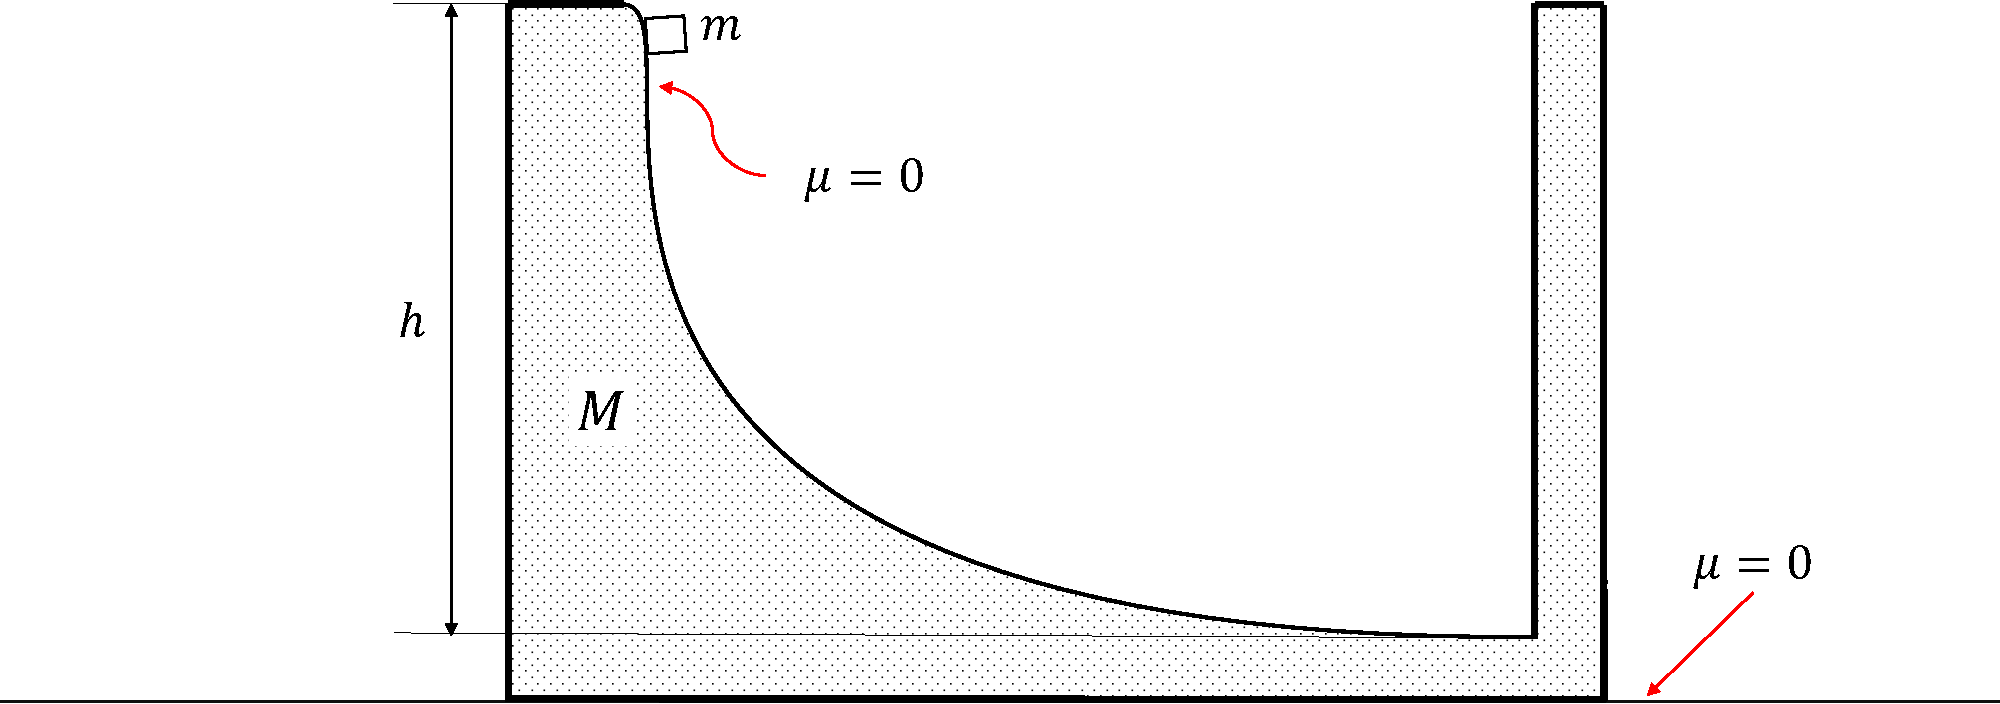
\includegraphics[width=0.5\linewidth]{2020-1/Imágenes/aux13/cuna.pdf}
\end{figure}

\item Una masa $m$ es soltada desde el punto más alto de un tazón semiesférico de radio $R$, encontrándose en su camino con otra masa de las mismas características, la cual está en reposo en el punto más bajo de aquel, quedando unidas tras el impacto. 
\begin{enumerate}
    \item Despreciando la fricción entre las masas y el tazón, determine la altura máxima alcanzada por el sistema. 
    \item Compare la energía de la situación inicial y final.
\end{enumerate}

\begin{figure}[H]
    \centering
    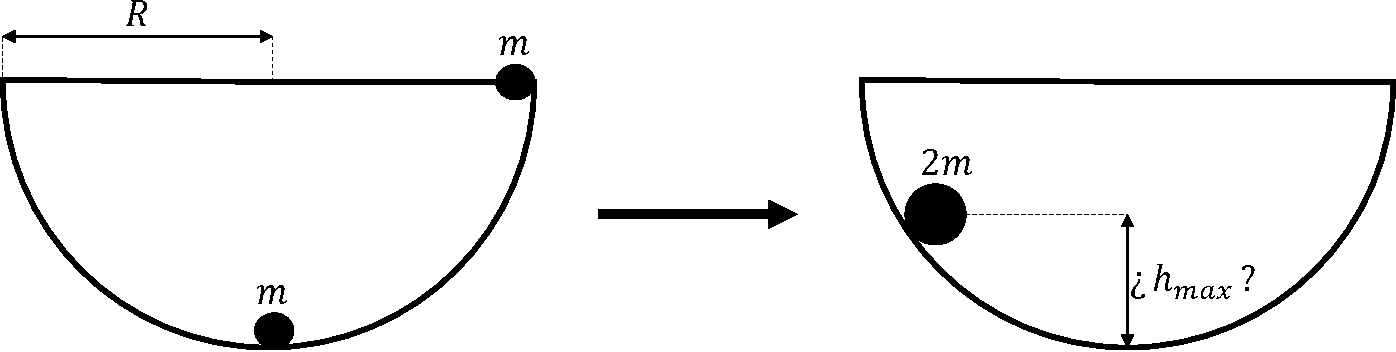
\includegraphics[width=0.5\linewidth]{2020-1/Imágenes/aux13/sem.pdf}
\end{figure}

\item Considere el montaje mostrado en la figura. Ambos bloques poseen masa $m$ y la distancia $l_0$ coincide con el largo natural del resorte de constante elástica $k = 5mg/l_0$. El bloque se desliza sin roce sobre la superficie y el sistema se encuentra inicialmente en reposo.

    \begin{enumerate}
        \item Determine la distancia horizontal que recorre el bloque en el cual comenzará a levantarse de la superficie
        
        \item Obtenga la rapidez del bloque en el punto anterior
    \end{enumerate}
    
\item Considere dos bloques de masa $m$ unidos por un resorte de constante elástica $k$. El sistema formado por los dos bloques y el resorte descansa en forma vertical sobre una mesa tal como lo indica la figura. ¿En cuánto debe comprimirse el resorte con respecto al largo natural para que al soltar el sistema, este eventualmente se despegue de la mesa?

\begin{figure}[H]
    \centering
    \svgpath{../Imagenes/aux11/}
    \begin{subfigure}[t]{0.45\textwidth}
        \centering
        \includesvg[width=0.65\linewidth]{wea.svg}
        \caption*{Figura P4}
    \end{subfigure}
    \hspace{0.1em}
    \begin{subfigure}[t]{0.45\textwidth}
        \centering
        \includesvg[width=0.5\linewidth]{wa.svg}
        \caption*{Figura P5}
    \end{subfigure}
\end{figure}

\item Una masa $M$ estpa atada al extremo de un resorte de constante elástica $k$ adosado a una pared. La masa desliza sobre un plano horizontal cuyo coeficiente de roce cinético es $\mu$ Inicialmente el resorte está comprimido una distancia $\delta_0$ con respecto a su posición ded equilibrio. En $t=0$ la masa se suelta, llegando a alcanzar el resorte una elongación máxima $\delta_1$, luegto vuelve y alcanza una elongación máxima $\delta_2$, y así sucesivamente. Encuentre una relación entre $\delta_{n+1}$ y $\delta_n$

\begin{figure}[htbp]
  \centering
  \svgpath{../Imagenes/aux11}
  \includesvg[width=0.5\linewidth]{resortepana.svg}
\end{figure}



\end{enumerate}
\end{document}
